% !TEX root =  manual.tex
\section{Statistical Theory}\label{sec:stattheory}
\subsection{References and Notation}

This is a brief description of the theory behind the emulator used here. For those more interested in details of the procedure, we refer you to the following references:
\begin{itemize}

\item F.~A.~Gomez, C.~E.~Coleman-Smith, B.~W.~O'Shea, J.~Tumlinson and R.~L.~Wolpert.
  ``Characterizing the formation history of Milky Way-like stellar halos with model emulators.''
	\emph{The Astrophysical Journal} {\bf 760}. 2 (2012) 112.
\url{http://iopscience.iop.org/0004-637X/760/2/112}
%  arXiv.org:1209.2142 [astro-ph.GA] (2012).

\item J.~Novak, K.~Novak, S.~Pratt, C.~E.~Coleman-Smith and R.~L.~Wolpert
  ``Determining Fundamental Properties of Matter Created in Ultrarelativistic Heavy-Ion Collisions,''
  arXiv:1303.5769 [nucl-th] (2013).
\url{http://arxiv.org/abs/1303.5769}

\item S.~Habib, K.~Heitmann, D.~Higdon, C.~Nakhleh and B.~Williams.
  ``Cosmic Calibration: Constraints from the Matter Power Spectrum and the Cosmic Microwave Background.''
  \emph{Phys.\ Rev.\ D} {\bf 76}. 8 (2007) 083503 .
\url{http://prd.aps.org/abstract/PRD/v76/i8/e083503}
  %[astro-ph/0702348 [ASTRO-PH]].

\item C.~E.~Rasmussen and C.~K.~I.~Williams, \emph{Gaussian Processes for Machine Learning}, The MIT Press (2005).
\url{http://www.gaussianprocess.org/}

\end{itemize}
\begin{table}[ht]
\begin{center}
\caption{Symbols used in this section}
\begin{tabular}{|c|l|}
\hline
$x_{i=1\cdots P}$& the $P$~{\rm model~parameters}\\
\hline
$y^{\rm(exp)}_{a=1\cdots M}$ & $M$ experimental measurements\\
\hline
$y^{\rm(mod)}_a({\bf x})$ & full-model values corresponding to the measurements\\
\hline
$z^{\rm(mod)}_a({\bf x})$ & PCA components, i.e., a rotation of ${\bf y}$.\\
\hline
$\sigma_a$ & the uncertainties associated with comparing $y^{\rm(exp)}_a$ to $y^{\rm(mod)}({\bf x})$\\
\hline
$X_{i,\alpha=1\cdots N}$ & parameter values of the $N$ training points\\
\hline
$Y_{a,\alpha}$ & observables as calculated at $N$ training points\\
\hline
$Z_{a,\alpha=1\cdots N}$ & model values of PCA components.\\
\hline
$\Theta_i$ & Hyper-parameters used by the emulator.\\
\hline
${\mathcal L}({\bf x})$ & likelihood for a specific point in parameter space to reproduce the data.\\
\hline
\end{tabular}
\end{center}
\end{table}

\subsection{Overview}

Markov Chain Monte Carlo (MCMC) explorations of the parameter space provide a sampling (perhaps millions) of points in the parameter space weighted by the likelihood, ${\mathcal L}({\bf x})$ where ${\mathcal L}$ represents the probability density for ${\bf x}$ to be the correct parameters given the experimental observations $Y^{\rm(exp)}_a$, or $P({\bf x}|{\bf Y})$. By Bayes theorem,
\begin{equation}
P({\bf x}|{\bf Y}^{\rm(exp)}) = \frac{P({\bf Y}^{\rm(exp)}|{\bf x}) P({\bf x})}{P({\bf Y}^{\rm(exp)})}.
\end{equation}
Since we will be doing sampling, we won't worry about normalizations, and since the measurements are what they are, we can neglect the $P({\bf Y}^{\rm(exp)})$ term in the denominator. The probability, $P({\bf x})$, of the parameter ${\bf x}$ in the absence of the experimental observations, ${\bf Y}^{\rm(exp)}$, is known as the prior. A common choice is a flat prior within a bounded space. The conditional probability $P({\bf Y}^{\rm(exp)}|{\bf x})$ is found by running the full model at ${\bf x}$, then comparing the model values to the corresponding experimental observations. A common choice for stating the probability is,
\begin{equation}
P({\bf Y}^{\rm(exp)}|{\bf x})\sim \exp\left\{-
\sum_a\frac{(Y^{\rm(exp)}_a-y_a^{\rm(mod)}({\bf x}))^2}{2\sigma_a^2}\right\}.
\end{equation}
Here, $\sigma_a$ is the uncertainty, or error, associated with comparing the experimental measurement to the model. This would encapsulate both the measurement error, aleatoric error (random errors due to finite statistics of either the measurement or of the model), and a measure of the trustworthiness of the theoretical treatment. One way to view $\sigma_a$ is to ask the question, ``If all the unknown physical parameters were correct, with what uncertainty do you believe your model would reproduce the experimentally reported value of $y_a$?''. The simple Gaussian form above could easily be replaced by a different functional form. For example, the form might have longer tails than a Gaussian, or one might replace the factor $1/\sigma_a^2$ with a matrix, i.e. correlated errors.

A straight-forward MCMC treatment would be to sample parameter space with the posterior probability, or likelihood, as calculated above.
\[
{\mathcal L}({\bf x})=P({\bf x}|{\bf y^{\rm(exp)}}).
\]
The most-used methods for creating MCMC traces is based on the Metropolis algorithm. This is a weighted random walk, where each step is accepted or rejected randomly with a probability proportional to the ratio of likelihoods at the two points if the new likelihood is lower, and is always accepted if the new likelihood is higher. However, this may require many millions of samplings for a multi-dimensional parameter space, and the model would need to be run at each point. If a model takes more than a few minutes, this procedure becomes untenable, and model emulators are required.

The model emulator's task is to reproduce the likelihood. The emulator is trained by some number, $N$, of full-model runs. Then, during the MCMC trace, the likelihood is determined by interpolating from the $N$ full-model runs, rather than by re-running the original model. Gaussian-Process (GP) based emulators are particularly popular, partly because they also provide an estimate of their accuracy. However, the reliability of this prediction, as well as the reliability of any scheme for interpolating or extrapolating, depends on the nature of the function being emulated. There is no substitute for detailed testing of the emualator.

Rather than emulating the likelihood directly, the models emulate a few principal components. In a principal component analysis (PCA) one finds the linear combinations, $z_a$, of the original observables $y_a$ that vary the most relative to the uncertainties $\sigma_a$. For the PCA analysis, one first scales the variables $y_a$ to new variables,
\[
\tilde{y}_a\equiv \frac{y_a-\langle y_a\rangle}{\sigma_a}.
\]
Here, $\langle \cdots\rangle$ refers to the average of the observable throughout the $N$ training runs, assuming the $N$ training runs are randomly chosen across the space. If the original error matrix were off-diagonal, one would first rotate the $y$s to a coordinate system where the error matrix was diagonal. The new observables $\tilde{y}$ are dimensionless and have uncertainties of unity. Next, one rotates to a coordinate system that diagonalizes the matrix $\langle \tilde{y}_a\tilde{y}_b\rangle$, which has eigenvalues $\lambda_a$. The coordinates are $z_a$, and are ordered by the size of $\lambda_a$. The new observables $z_a$ also have uncertainties of unity, and vary throughout the parameter space by an amount $\sqrt{\lambda}$. Those components with $\lambda_a\gtrsim 1$ are effective at constraining the parameter space, while those with $\lambda_a\ll 1$ have little effect and can be set to zero without significantly affecting the likelihood. I.e., if one sets these components to zero and rotates from ${\bf z}$ back to $\tilde{\bf y}$, the value of $\tilde{y}$ will be the same as if ${\bf z}$ were some small fraction of unity. Thus, the main purpose of PCA is to identify a few effective observables to emulate that carry the great majority of the resolving power. One can also rotate the experimental values $y_a^{\rm(exp)}$ to the new system and find $z_a^{\rm(exp)}$. In the Gaussian form for the likelihood above, one then finds
\[
{\mathcal L}({\bf x})\sim \exp\left\{-\frac{1}{2}\sum_a(z^{\rm(mod)}_a({\bf x})-z_a^{\rm(exp)})^2\right\}.
\]
Only those components that have significant values of $\lambda$ need be considered.

An obvious question is ``Why not just emulate the likelihood? -- rather than emulating several principal components''. The motivation comes from the fact that it is inherently more difficult to interpolate a function near it's maximum. Near the point of maximum likelihood, the PCA components are still likely to be acting monotonically in the region of interest. The maximum of ${\mathcal L}$ then comes from the fact that the principal components, $z_a$, contribute quadratically to the likelihood.

\subsection{Sample runs for Emulator Training}
One wishes to choose the $N$ training points in a way which best spans the space. Additionally, one wishes to ensure that the choice avoids reusing individual components. For example, consider $N=27$ points chosen to span a three-dimensional parameter space, $x_1,x_2$ and $x_3$. Once could divide the space into 27 sub cubes, then place one point in the center of each sub-cube. However, only three values of $x_1$ would be sampled. If the model were insensitive to $x_2$ and $x_3$, the calculation would essentially only use three values to construct the resulting function of $x_1$. Latin hyper-cube sampling would divide the cube into $N\times N\times N$ sub cells, then populate the cells in a way that ensures that no two populated cells share any component. A two-dimensional example is illustrated in Fig. \ref{fig:hypercube}

\noindent
\begin{figure}
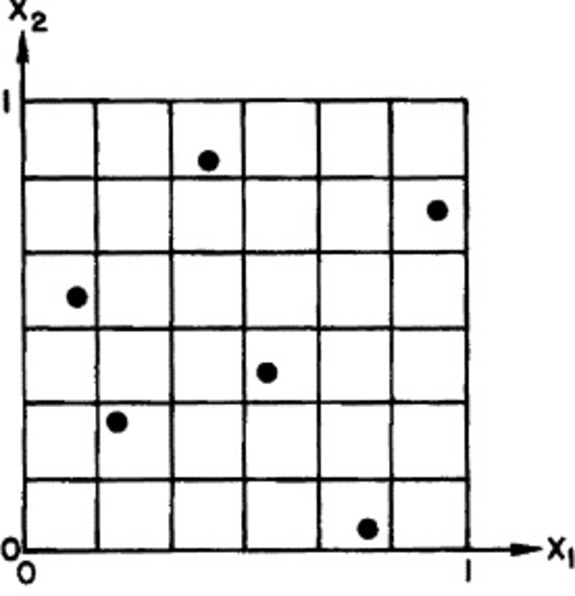
\includegraphics[width=2.5in]{figs/hypercube}
\parbox[b]{4.5in}
{\caption{\label{fig:hypercube}
Latin hyper-cube sampling is illustrated here with $N=8$ points in a two-dimensional parameter space. No two populated cells have the same value for either $x_1$ or $x_2$.}
\vspace*{60pt}
}

\end{figure}

Before executing the $N$ sample runs of the full model, one must first choose the parameter values $X_{i,\alpha}$, where $i=1\cdots P$ labels the specific parameter (e.g. the temperature) and $\alpha=1\cdots N$ refers to the specific run. For parameters with uniform distributions in fixed intervals, the usual choice is to pick parameters according to {\it Latin hyper-cube} sampling (LHS). In LHS each of the $P$ parameters are divided into $N$ slices. The $N$ points in parameter space are then chosen so that $X_{i,\alpha}$ and $X_{i,\beta}$ never come from the same slice.
%% The algorithm also attempts to uniformly cover the entire space and
%% ensure that $X_{\alpha}$ is never close to $X_{\beta}$.
A special tool is provided to generate a set of parameters. If you provide a file listing the parameter names and their ranges the tool will provide $N$ files listing the parameter values for each of the $N$ runs.

Once you have the model parameters, the next step is to run the model at each point and store the results. Typically, model output produces MANY more values than the $M$ values for $y_{a=1\cdots M,\alpha}$ at each model point. For instance, the model might produce 40 values describing a spectra as as function of momentum or frequency. However, it is most likely untenable to build emulators for all 40 values. Instead the spectra might be summarized by a few numbers, such as the new yield (integrated area under the curve) or the mean momentum or mean frequency. The modeler typically has a good understanding of which, and how many, values are required to distinguish the spectra from other spectra created from different model runs. One could do a principal component analysis (PCA) to best determine such parameter, or perhaps to justify the number of such parameters. Unless there is a strong motivation, it is preferable to use values that have a clear physical understanding (such as yield) and to stay away from obtuse linear combinations of disparate values. Since PCA analyses will be performed later on, it is better to error on the side of too-many parameters at this point.

Thus the model run may consist of two steps, first running the model $N$ times to produce a fairly large output, and secondly performing a distillation to what may be on the order of dozens or hundreds of observables $Y_{a,\alpha}$.

\subsection{Emulator Theory}

The goals of the emulator are:
\begin{itemize}
\item[a)] Give a best estimate for ${\bf y}^{(\rm emu)}({\bf x})$ for any point ${\bf x}$ in parameter space based on the $N$ samplings, ${\bf Y}_\alpha={\bf y}^{\rm(mod)}({\bf X}_\alpha)$. Again the dimension of $x$ is the number of parameters $P$ and the dimension of the vector ${\bf y}$ is the number of observables $M$.
\item[b)] The emulator should also provide an estimate of it's own error.
\end{itemize}

In order to build the emulator, one first performs a PCA (Principle Component Analysis). This involves finding linear combinations of the $M$-dimensional vectors $y$ such that the new vectors $M$-dimensional vectors ${\bf z}$ have a diagonalized variance within the sampling space. After one orders the $M$ components according to the amount of their variance throughout the sampling space, one can discard all those components that have small variance. I.e., ``observables'' that do not vary throughout the sampling space can be emulated as fixed numbers, so one needn't devise a sophisticated emulator for them. The non-discarded components are referred to as principal components.

\subsubsection{Principal Component Analysis}

Before embarking on the PCA analysis, we first restate the observables $y_i$ by subtracting the mean and dividing by $\sigma_i$. The resulting values are
\begin{equation}
\tilde{y}_a\equiv\frac{y_a-\bar{y}_a}{\sigma_a}.
\end{equation}
Since ${\bf y}$ is sampled rather uniformly by the LHS sampling, the averages, $\bar{y}_a$, can be taken as the average from the $N$ sampling runs. Dividing by $\sigma_i$ is necessary to create a quantity that is dimensionless, and to give meaning to the variation. For instance, when investigating the variance of $y_a$ amongst the model runs, the observable would only provide decent resolving power if the r.m.s. variance is of the order or greater than $\sigma_a$. With this definition, one can state that only those components $\tilde{y}_a$ that vary of order unity or greater can affect the answer. We will be rotating the vectors $\tilde{\bf y}$ in the PCA analysis to create new vectors ${\bf z}$, with each component $z_a$ being a linear combination of the components $\tilde{y}_a$. It would make no sense to take linear combinations of the un-scaled components $y_i$ because they have different units.

The $M\times M$ covariance matrix is determined from the $N$ sampling runs,
\begin{equation}
\Xi_{ab}=\frac{1}{M}\sum_\alpha \tilde{Y}_{a,\alpha}\tilde{Y}_{b,\alpha}.
\end{equation}
The matrix $\Xi$ has eigenvalues $\lambda^{\rm(c)}$ and normalized eigenvectors $\xi_b^{\rm(c)}$,
\begin{equation}
\label{eq:Xidef}
\Xi_{ab}\xi_b^{\rm(c)}=\lambda^{\rm(c)} \xi_b^{\rm(c)}.
\end{equation}
The principal components, $z_a$, are unitary transformations of the vectors $\tilde{y}_a$, with the transformation matrix given by the eigenvectors,
\begin{eqnarray}
\label{eq:pcarotation}
z_a&=&U_{ab} \tilde{y}_b,\\
\nonumber
U_{ab}&=&\xi_b^{\rm(a)},~~U^{-1}_{ab}=U_{ba}.
\end{eqnarray}
After calculating $\Xi$ from the samplings $\tilde{Y}_a$, then performing the matrix algebra to find the eigenvalues and eigen-vectors, one can rotate $\tilde{Y}_{a,\alpha}$ to obtain $Z_{a,\alpha}$, the principal components for each of the sampling points. However, instead of emulating all $M$ components of $z_a$ at some new point ${\bf x}$, one need only emulate the first several, while setting the remainder to zero. One then transforms ${\bf z}^{\rm(emu)}({\bf x}$ to ${\bf y}^{\rm(emu)}({\bf x})$ with the transformation $U^{-1}$ defined above.

\subsubsection{Gaussian Process (GP) Emulators}

One can choose from a large class of emulators. Any scheme for estimating $z_a({\bf x})$ from the samplings $Z_{a,\alpha}$ taken at $N$ points ${\bf x}_\alpha$ can serve as an emulator. This could include schemes a simple as a linear or quadratic fit. These simple fits can also provide an estimate of the error if one considers the average deviation from the fit. However, fitting functions is dangerous if one does not have a good understanding of the appropriate functional form. Further, it can be advantageous to have an interpolative scheme, i.e., one that goes through all the $N$ training points. The GP emulator provides a smooth interpolation that exactly reproduces the training points, even in a high dimensional space with randomly located training points.

The GP emulator considers the correlation between the emulated function, $z$, between any two points ${\bf x}_i$ and ${\bf x}_j$ (Since we emulate the components $z_a$ one-at-a-time, we can drop the subscript $a$). The correlation is assumed to have a form, e.g.,
\begin{eqnarray}
\label{eq:hyperform}
c({\bf x}_i,{\bf x}_j)&\equiv&\langle z({\bf x}_i)z({\bf x}_j)\rangle\\
\nonumber
&=&\Theta_0\exp\left\{-\frac{1}{2}\sum_k^P \frac{(x_{1,k}-x_{2,k})^\alpha}{2\Theta_k}\right\} +\delta_{ij}\Theta_N,
\end{eqnarray}
where the average denotes the average over all possible functions that have this correlation. The quantities, $\Theta_0\cdots\Theta_N$ and $\alpha$ are referred to as {\it hyper-parameters}. The final term, $\delta_{ij}\Theta_N$, which give a correlation only between a point and itself, is known as a nugget. It accounts for point-by-point noise

Solving for the most probable value for the $z({\bf x})$ given the training values, $Z_\alpha$, one can find
\begin{eqnarray}
z^{\rm(emu)}({\bf x})&=&\sum_{\alpha\beta}c({\bf x},{\bf X}_\alpha) C^{-1}_{\alpha\beta}Z_\beta,\\
\nonumber
C_{\alpha\beta}&=&c({\bf x}_\alpha,{\bf x}_\beta).
\end{eqnarray}
If the function is first fit to some function, e.g. a linear fit, one can choose to emulate only the difference. If the point ${\bf x}$ approaches one of the training points,
\begin{eqnarray}
z^{\rm(emu)}({\bf x}_\alpha)&=&\sum_{\beta\gamma}c({\bf x}_\alpha,{\bf x}_\beta) C^{-1}_{\beta\gamma}Z_\gamma\\
\nonumber
&=&\sum_{\beta\gamma}C_{\alpha\beta}C^{-1}_{\beta\gamma}Z_\gamma=Z_\alpha.
\end{eqnarray}
The last step ignored the nugget term, which breaks the equality, i.e. $c({\bf x}\rightarrow {\bf X}_\alpha,{\bf X}_\alpha)\ne c({\bf X_{\alpha},{\bf x}_\alpha})$. Thus, the emulator returns the training value if ${\bf x}$ is chosen to equal one of the training points, but only if the nugget term is zero. Since the emulated functions are continuous (and smooth if $\alpha=2$) the GP emulator can be thought of as an interpolator that works for multidimensional functions.

A handy feature of the GP emulator is that it also provides an estimate of it's own error,
\begin{equation}
\sigma^2({\bf x}) = c({\bf x},{\bf x}) -\sum_{\alpha\beta}c({\bf x},{\bf X}_\alpha)C^{-1}_{\alpha\beta}
c({\bf X}_\beta,{\bf x}).
\end{equation}
If one neglects the nugget term, one can see that in the limit that ${\bf x}$ approaches, but does not exactly equal, a training point ${\bf X}_\alpha$, $\sigma^2$ goes to zero. Including the nugget leads to $\sigma^2>0$ even for values of ${\bf x}$ approaching a training point. If one understands the point-by-point randomness of $z^{\rm(mod)}$, e.g., let's assume $z$ is calculated using a stochastic model and has an uncertainty $\sigma^{\rm(mod)}$, the hyper-parameter $\Theta_N$ should be set equal to $\sigma^{{\rm(mod)},2}$. If $z^{\rm(mod)}$ is calculated by the model without aleatoric error, $\Theta_N$ should be set to zero. As long as $\sigma$ is set to a number rather smaller than unity, it should have little if any effect, and might even enhance the numerical stability.

The other hyper-parameters can be chosen according to a variety of criteria. In Rasmussen, it is shown how to choose optimized parameters. However, our experience with this procedure is mixed, as the procedure might produce unreasonable estimates of it's error if the correlation does not truly have the functional form presumed. One might choose the hyper-radii, $\Theta_1\cdots\Theta_p$ to match length scales inherent in the model. Or, in the case where the model behaves smoothly and can be evaluated with a Taylor expansion, one might choose the radii to be some fraction, say half, of the overall parameter range. The hyper-parameter $\Theta_0$ is interesting because it does not affect the interpretation of $z^{\rm(mod)}$ (when $\Theta_N=0$), but it does affect the error estimate.

As an example of an emulated function, Fig. \ref{fig:emuexample} shows several functions in the right-hand panel, each of which are consistent with a Gaussian correlation structure as described in Eq. (\ref{eq:hyperform}). These were generated by taking a sum of Gaussians centered randomly about different points, effectively correlated noise. The left-hand panel shows the value and ranges that come from the emulator.
\begin{figure}
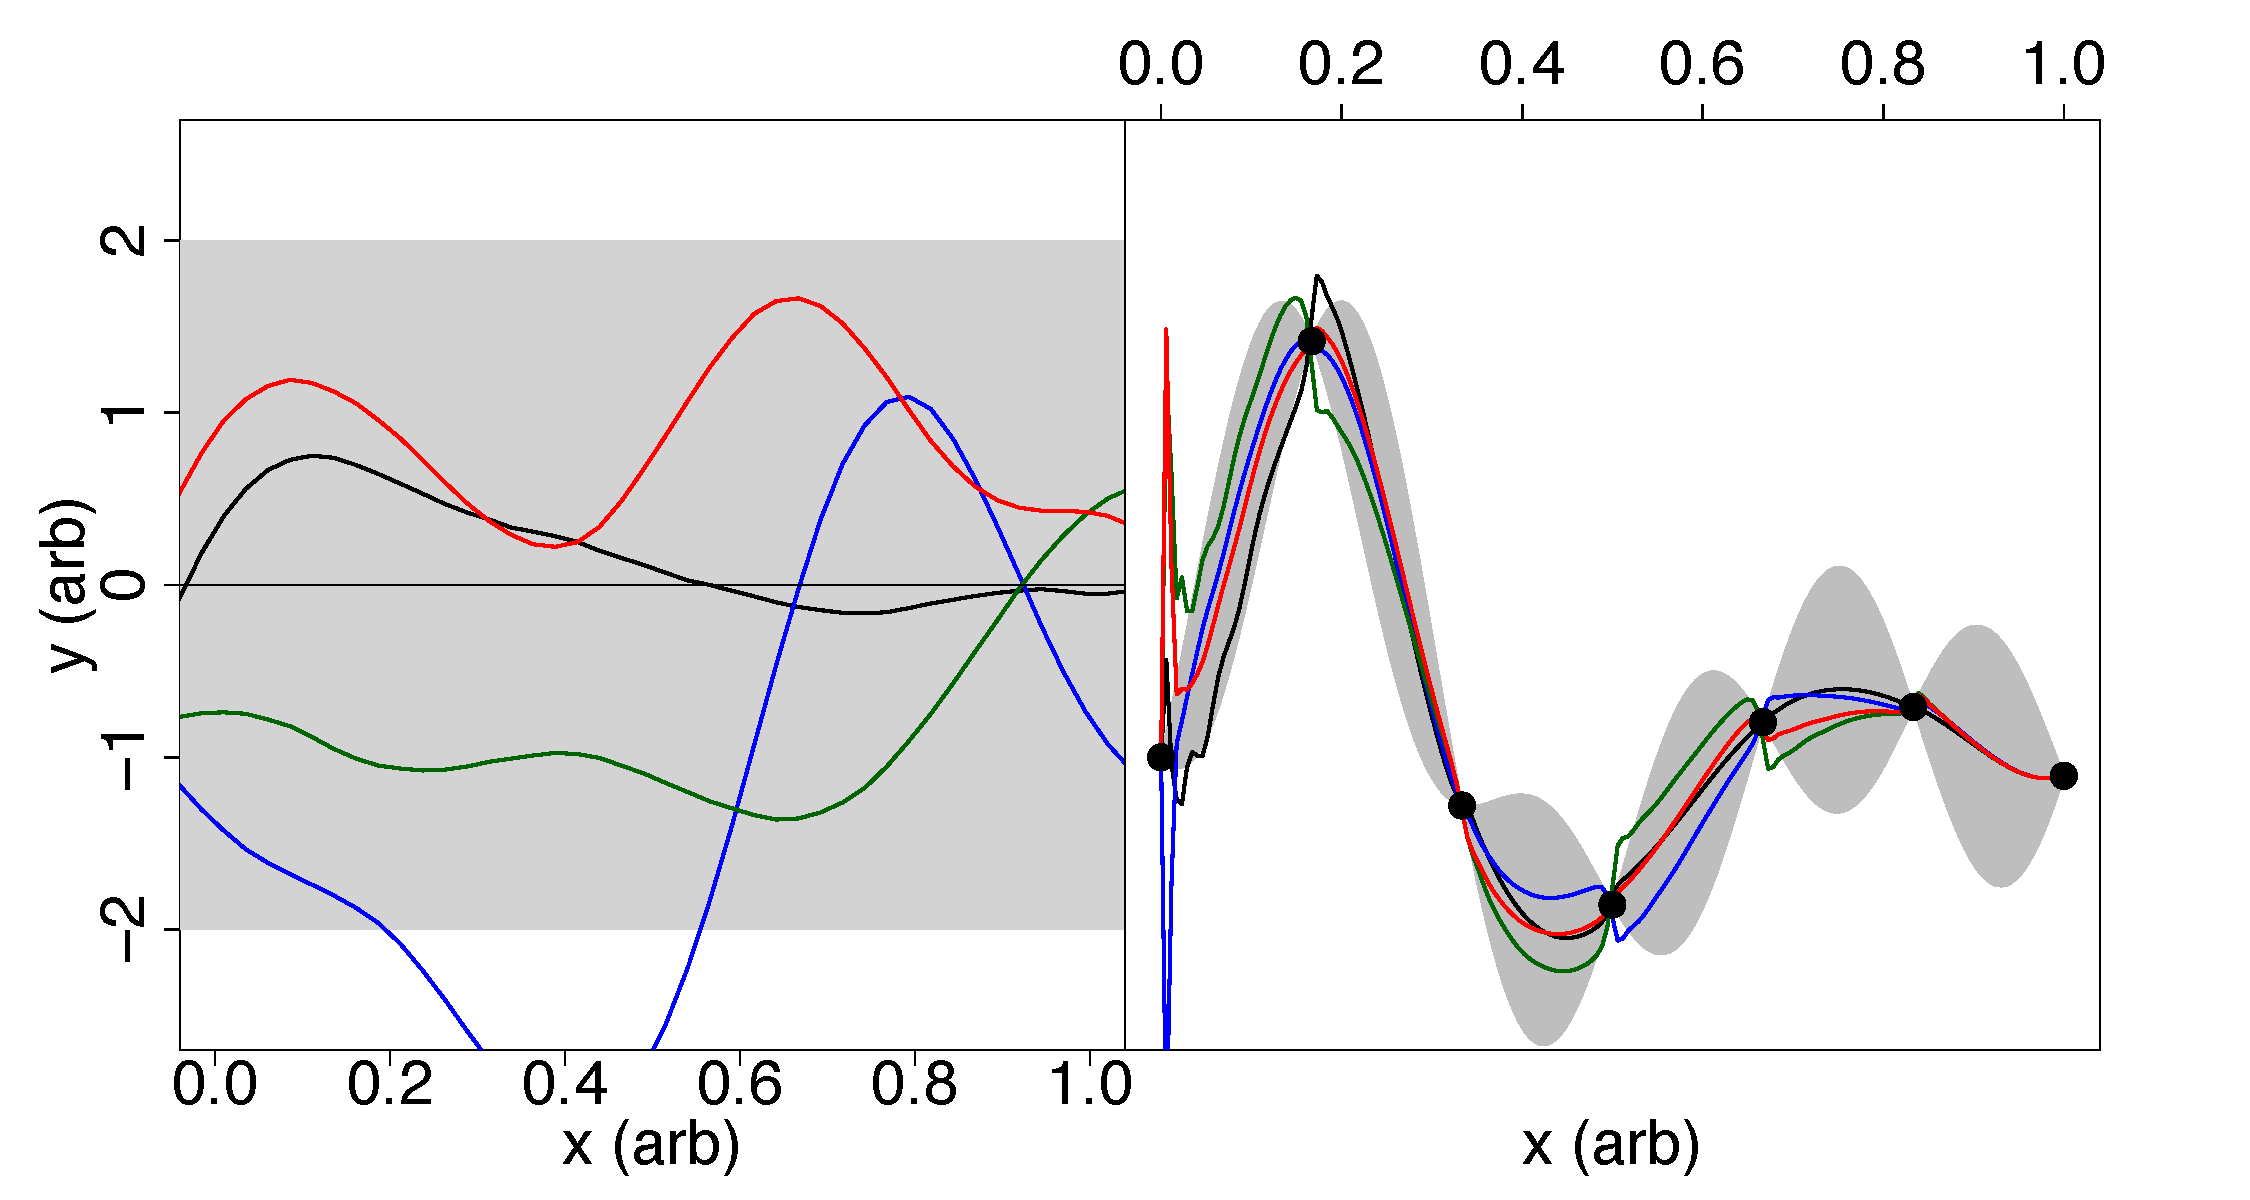
\includegraphics[width=4in]{figs/gaussian-reals-joined.pdf}
\parbox[b]{3.0in}{\caption{\label{fig:emuexample}
Left panel: Assortment of functions that have the covariance of the form assumed in Eq. (\ref{eq:hyperform}). The curves are created by taking a sum of Gaussians randomly centered about different points. Right panel: After training on 7 points, the gray bands show the 95\% confidence interval for predicting the values. The four curves in the r.h.s. represents four functions that are consistent with both the functional form and with the 7 sampled values.}}
\end{figure}

Our experience is that GP emulation provides a remarkably good tool for emulating and extrapolating values for $z^{\rm(mod)}$. Furthermore, the extrapolated values are often remarkably insensitive to how one chooses the hyper-radii as long as the radii are not much different than some scale at which the function changes, and if the function is smooth (only a few terms of a Taylor expansion are needed to describe the function) choosing radii of roughly half the overall extent of the parameter space seems to work well. However, despite being pretty reliable for reproducing the actual functions, GP emulators can be unreliable in providing an estimate of their own error, unless the assumed functional form come close to the truth. This is not true for functions with long-range trends, such as monotonically rising, semi-linear functions. If one anticipates such behavior, it is best to first perform a linear fit, then emulate the residual. The most reliable method for determining the accuracy of the emulator is to perform a handful of model runs with points not used to train the model, then check to see how well the emulator reproduced the model values.






